\title{Laporan Tugas Akhir}
\author{Fitri, Lintang}

\documentclass[12pt,twoside]{book}
\usepackage[a4paper,top=30mm,left=30mm,right=20mm,bottom=25mm]{geometry}
\usepackage[onehalfspacing]{setspace}
\usepackage[indonesian]{babel}
\usepackage{mathptmx}
\usepackage[pdfauthor={\@author},bookmarksnumbered,pdfborder={0 0 0}]{hyperref}
\usepackage[utf8]{inputenc}
\usepackage[table,xcdraw]{xcolor}
\usepackage[authoryear]{natbib}
\usepackage{amsmath}
\usepackage{caption}
\usepackage{verbatim}
\usepackage{tocloft}
\usepackage{changepage}
\usepackage{csvsimple}
\usepackage{enumitem}
\usepackage{eso-pic}
\usepackage{etoolbox}
\usepackage{subcaption}
\usepackage{graphicx}
\usepackage{hhline}
\usepackage{import}
\usepackage{lipsum}
\usepackage{lmodern}
\usepackage{longtable}
\usepackage{multido}
\usepackage{multirow}
\usepackage{pdflscape}
\usepackage{pdfpages}
\usepackage{rotating}
\usepackage{rotfloat}
\usepackage{tabularx}
\usepackage{wrapfig}
\usepackage{xpatch}
\usepackage{zref-abspage}
\usepackage{zref-user}


\renewcommand{\cftdotsep}{0.75} % Mengurangi jarak titik-titik
% \setlength{\cftbeforesecskip}{0.1pt} % Jarak sebelum section
% \setlength{\cftbeforesubsecskip}{0.1pt} % Jarak sebelum subsection
% \setlength{\cftbeforesubsubsecskip}{0.1pt} % Jarak sebelum subsubsection
\renewcommand{\cfttoctitlefont}{\hfill\bfseries\large} % Centers the title
\renewcommand{\cftaftertoctitle}{\hfill} % Ensures proper centering
\renewcommand{\listfigurename}{DAFTAR GAMBAR}
% \renewcommand{\cftbeforeloftitle}{\hfill}  % Add spacing before title
% \renewcommand{\cftafterloftitle}{\hfill}   % Add spacing after title% \renewcommand{\cftlistfigurename}{\hfill DAFTAR GAMBAR \hfill}
% \renewcommand{\cftlisttablename}{\hfill DAFTAR TABEL \hfill}

\patchcmd{\cleardoublepage}{\hbox{}}{
  \thispagestyle{empty}
  \vspace*{\fill}
  % \begin{center}\textit{[Halaman ini sengaja dikosongkan]}\end{center}
  \vfill
}{}{}

\usepackage{fancyhdr}
\fancyhf{}
\renewcommand{\headrulewidth}{0pt}
\pagestyle{fancy}
\fancyfoot[RO,LE]{\thepage}
\patchcmd{\chapter}{plain}{fancy}{}{}
\patchcmd{\chapter}{empty}{plain}{}{}

\usepackage{titlesec}
\titleformat{\chapter}[display]{\bfseries\large}{BAB \centering\Roman{chapter}}{0ex}{\vspace{0ex}\centering}
\titleformat{\section}{\bfseries\normalsize}{\MakeUppercase{\thesection}}{1ex}{\vspace{1ex}}
\titleformat{\subsection}{\bfseries\normalsize}{\MakeUppercase{\thesubsection}}{1ex}{}
\titleformat{\subsubsection}{\bfseries\normalsize}{\MakeUppercase{\thesubsubsection}}{1ex}{}
\titlespacing{\chapter}{0ex}{0ex}{4ex}
\titlespacing{\section}{0ex}{1ex}{0ex}
\titlespacing{\subsection}{0ex}{0.5ex}{0ex}
\titlespacing{\subsubsection}{0ex}{0.5ex}{0ex}

\usepackage{listings}
\renewcommand{\lstlistingname}{Kode}
\definecolor{comment}{RGB}{0,128,0}
\definecolor{string}{RGB}{255,0,0}
\definecolor{keyword}{RGB}{0,0,255}
\lstdefinestyle{code}{
  commentstyle=\color{comment},
  stringstyle=\color{string},
  keywordstyle=\color{keyword},
  basicstyle=\footnotesize\ttfamily,
  numbers=left,
  numberstyle=\tiny,
  numbersep=5pt,
  frame=lines,
  breaklines=true,
  prebreak=\raisebox{0ex}[0ex][0ex]{\ensuremath{\hookleftarrow}},
  showstringspaces=false,
  upquote=true,
  tabsize=2,
}
\lstdefinestyle{inline}{
  breaklines=true,
  prebreak=\raisebox{0ex}[0ex][0ex]{\ensuremath{\hookleftarrow}},
  showstringspaces=true,
  upquote=true,
  tabsize=2,
}
\lstset{style=inline}

\usepackage{pgfplots}
\pgfplotsset{compat=1.18}

\newcounter{cntsideways}
\makeatletter

\AddToShipoutPictureBG{
  \if@mainmatter
    \ifnum\zref@extractdefault{rotate\number\value{page}}{page}{0}=0
      \PLS@RemoveRotate
    \else
      \checkoddpage
      \ifoddpage
        \PLS@AddRotate{90}
      \else
        \PLS@AddRotate{-90}
      \fi
    \fi
  \fi
}

\newcommand\rotatesidewayslabel{
  \stepcounter{cntsideways}
  \zlabel{tmp\thecntsideways}
  \zlabel{rotate\zref@extractdefault{tmp\thecntsideways}{page}{0}}
}

\makeatother

\xapptocmd{\sidewaysfigure}{\rotatesidewayslabel}{}{}
\xapptocmd{\sidewaystable}{\rotatesidewayslabel}{}{}

\subimport{pustaka}{tanda-hubung.tex}

% \newenvironment{cover}[1]{
%   \AddToShipoutPictureBG*{
%     \AtPageLowerLeft{
%       \hspace{-3.5mm}
%       \raisebox{0mm}{
%         \includegraphics[width=\paperwidth,height=\paperheight]{#1}
%       }
%     }
%   }
%   \thispagestyle{empty}
%   \newgeometry{top=95mm,left=25mm,right=20mm,bottom=25mm}
%   \begin{flushleft}
%     \sffamily
%     \fontseries{bx}
%     \selectfont
% }{
%   \end{flushleft}
%   \restoregeometry
% }

\begin{document}

  \frontmatter
  
  % \begin{cover}{sampul/gambar/sampul-luar.png}
  %   \color{white}
  %   \subimport{sampul}{sampul-id.tex}
  % \end{cover}
  % \setcounter{page}{1}

  % \begin{cover}{sampul/gambar/sampul-dalam.png}
  %   \subimport{sampul}{sampul-id.tex}
  % \end{cover}
  % \cleardoublepage

  % \begin{cover}{sampul/gambar/sampul-dalam.png}
  %   \subimport{sampul}{sampul-en.tex}
  % \end{cover}
  % \cleardoublepage

  \phantomsection
  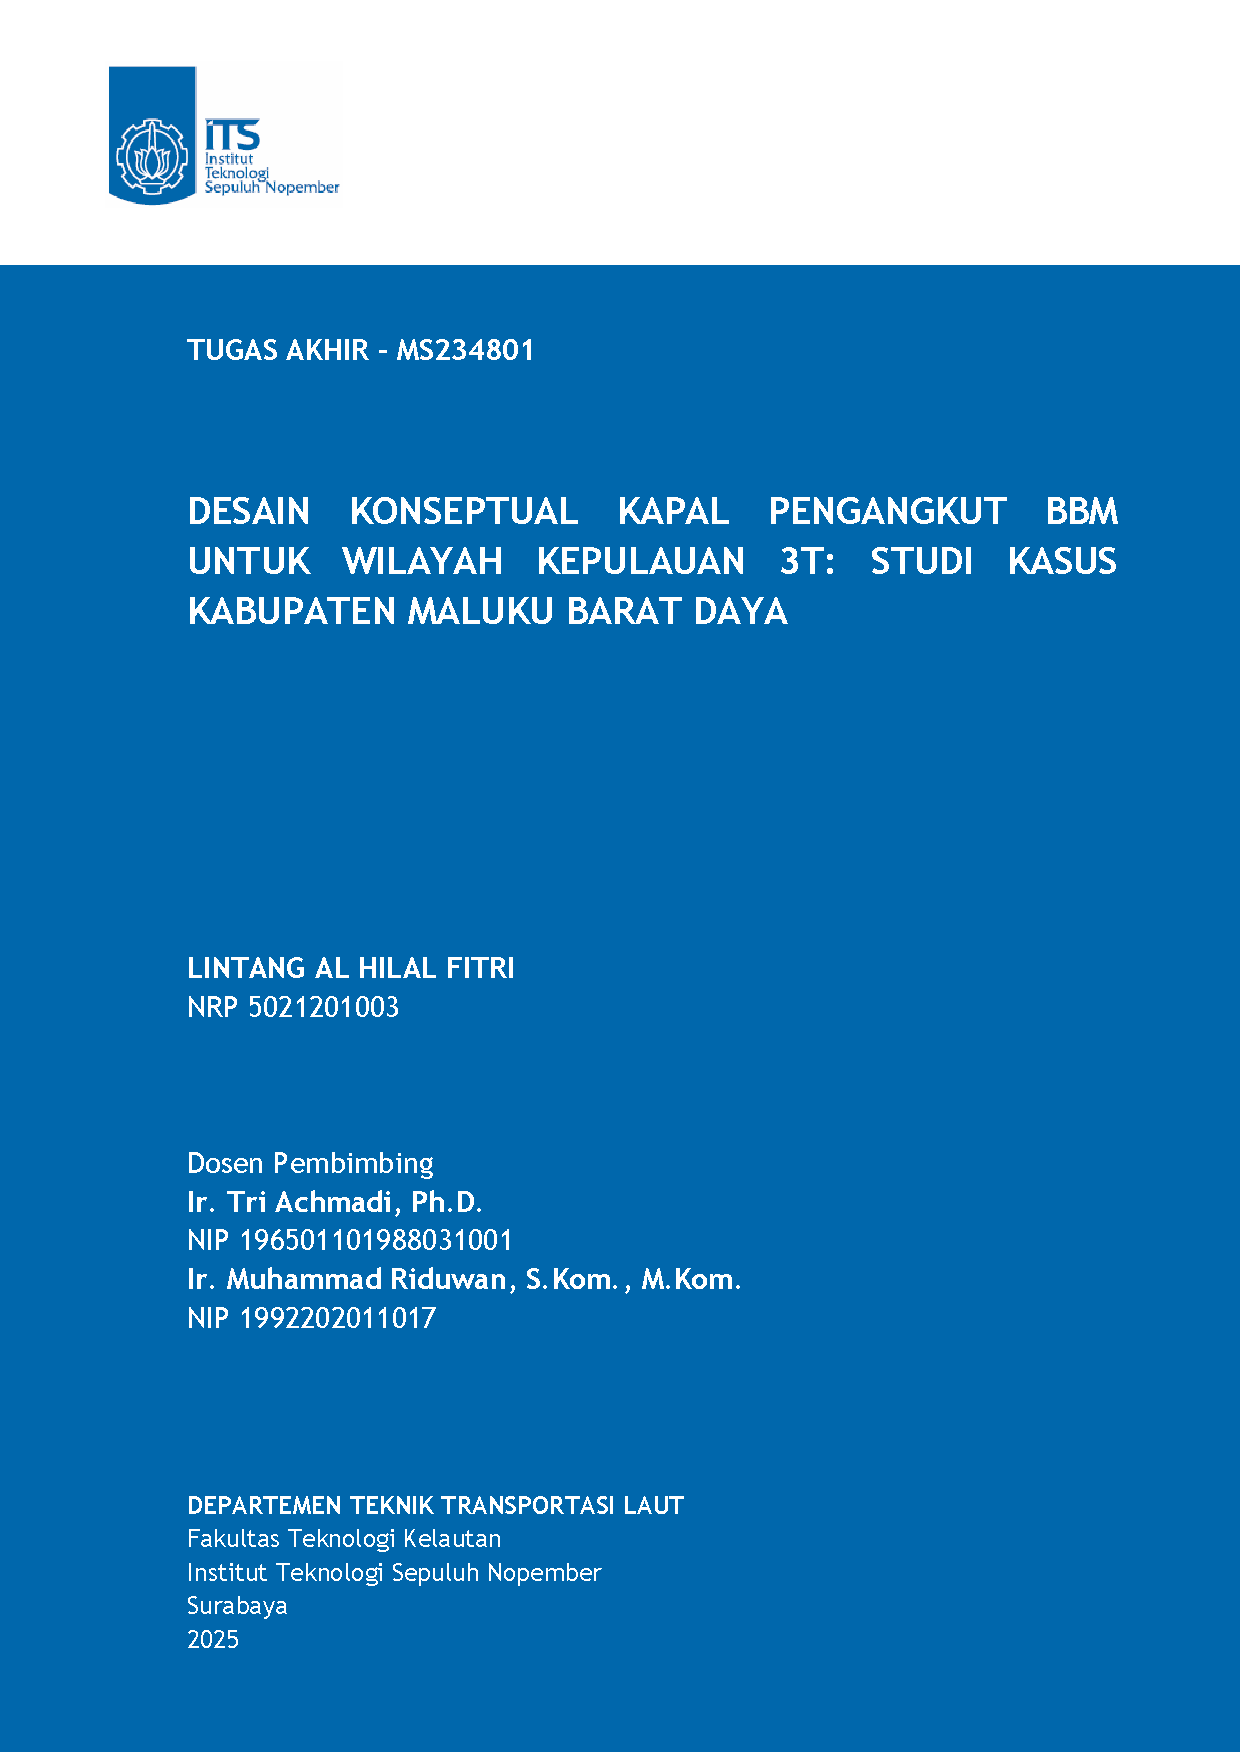
\includepdf[pages=-]{lainnya/sampul_luar.pdf}
  \cleardoublepage

  \phantomsection
  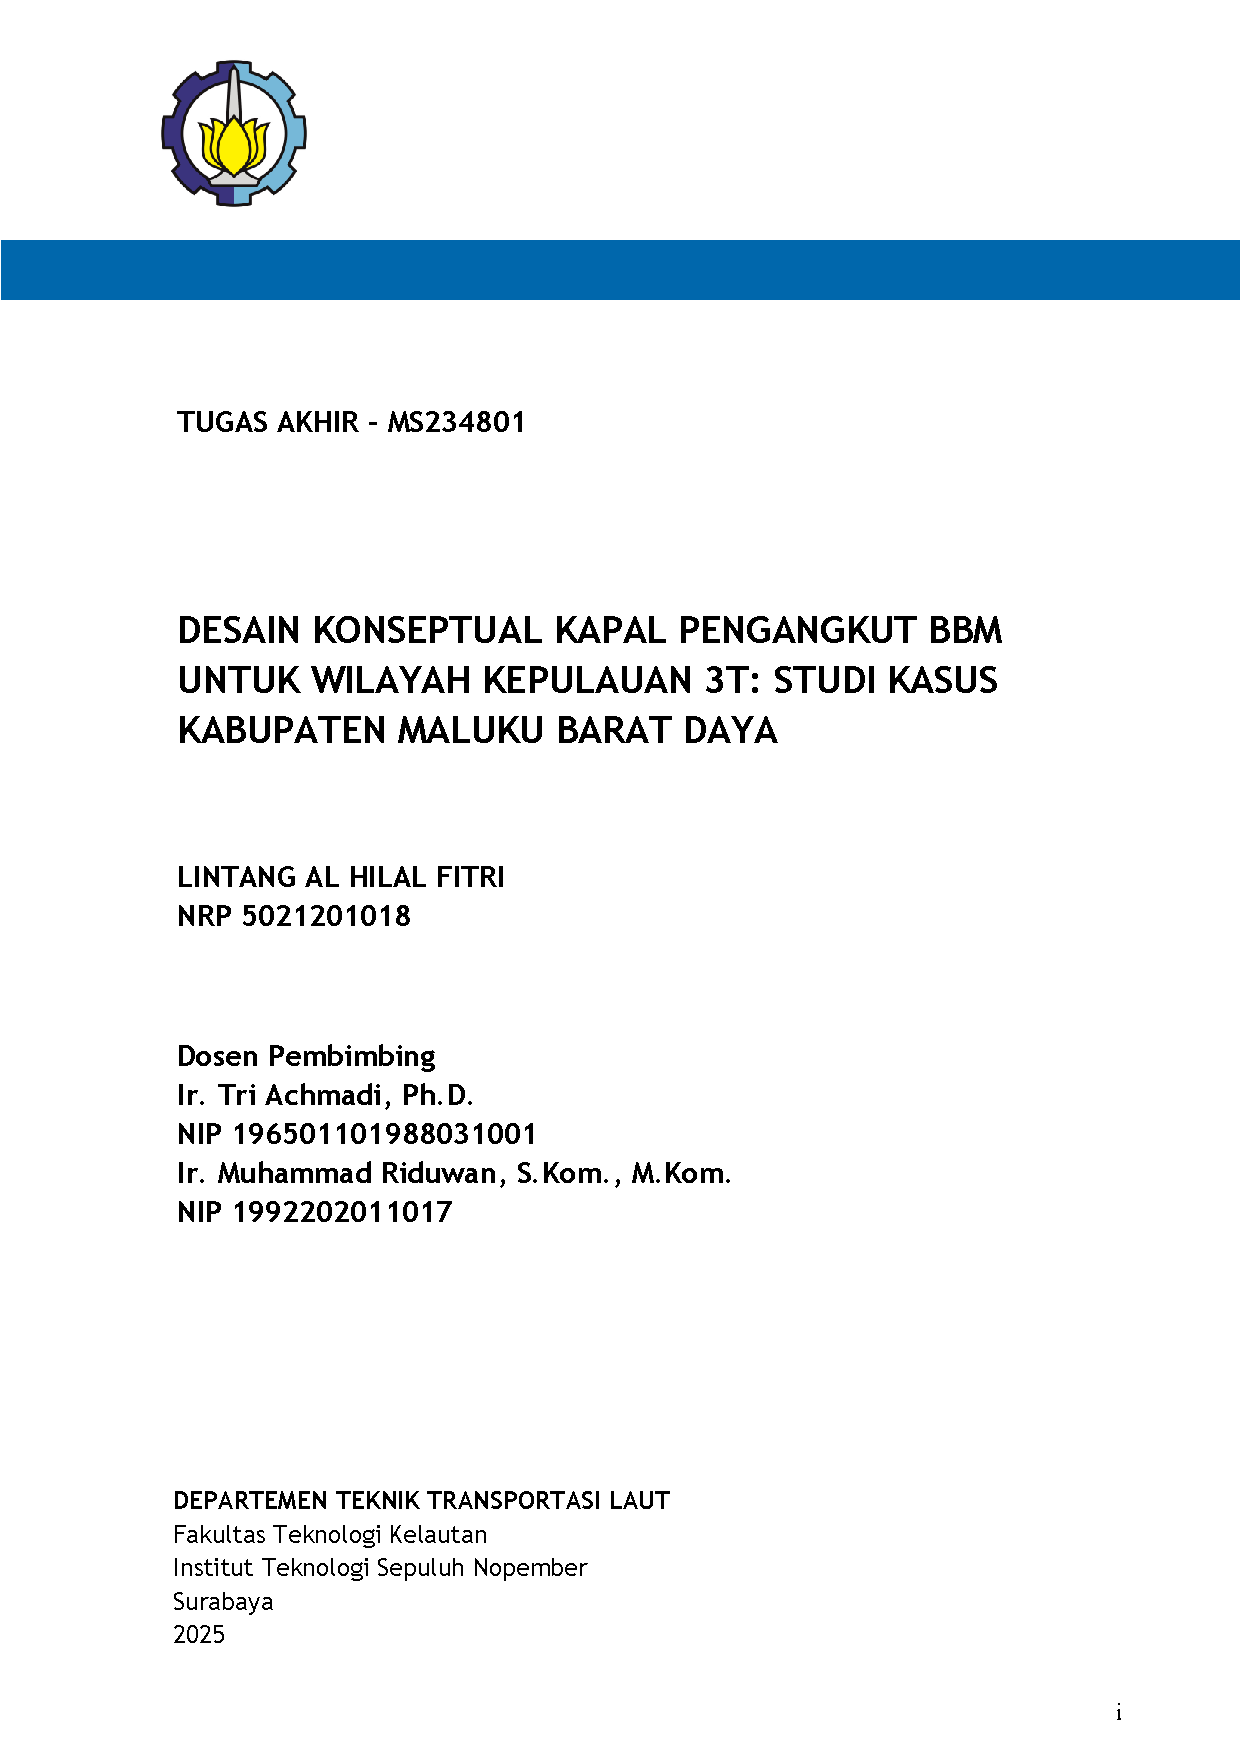
\includepdf[pages=-]{lainnya/sampul_dalam_id.pdf}
  \cleardoublepage

  \phantomsection
  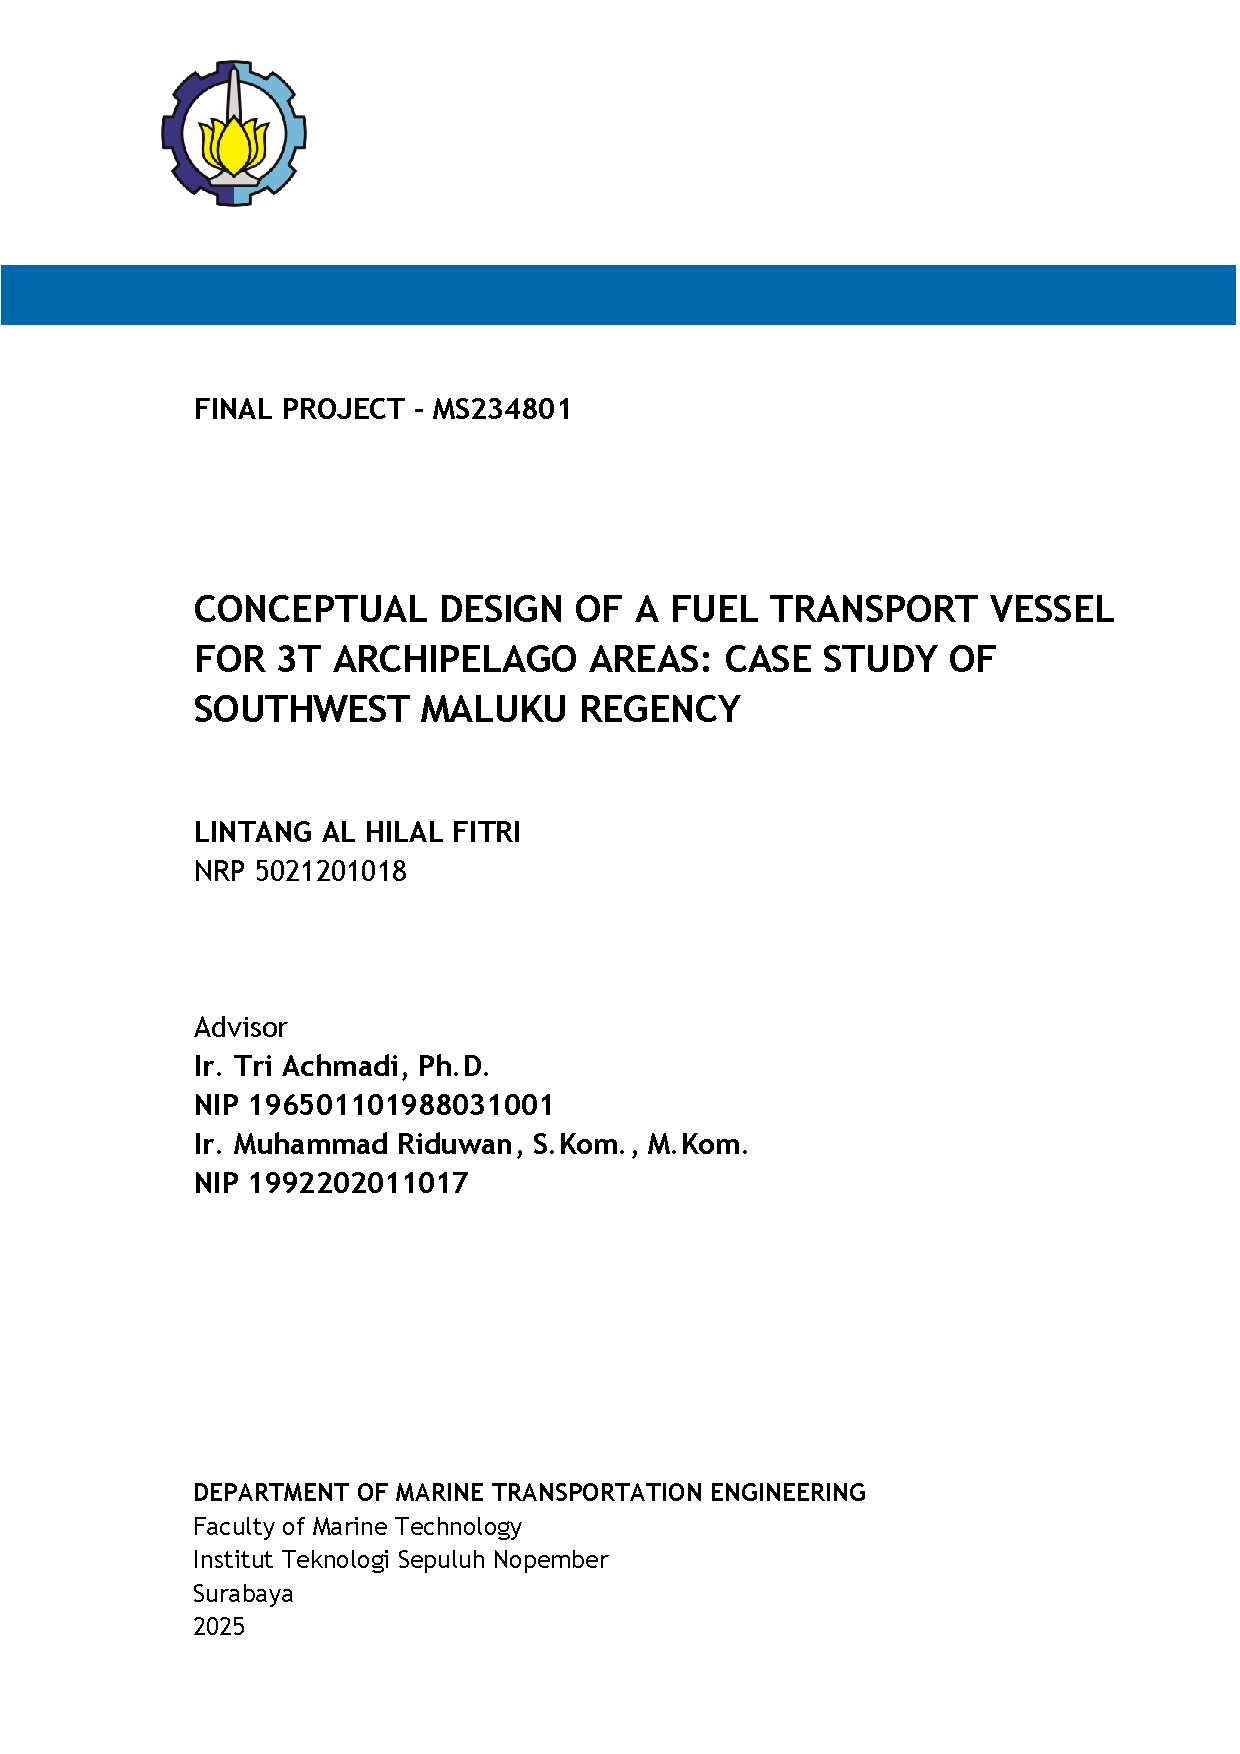
\includepdf[pages=-]{lainnya/sampul_dalam_en.pdf}
  \cleardoublepage

  \setlength{\parindent}{2em}
  \setlength{\parskip}{1ex}

  \phantomsection
  \addcontentsline{toc}{chapter}{LEMBAR PENGESAHAN}
  \includepdf[pages=-]{kep_yudisium/Approval.pdf}
  \cleardoublepage

  \phantomsection
  \addcontentsline{toc}{chapter}{PERNYATAAN ORISINALITAS}
  \includepdf[pages=-]{kep_yudisium/orisinalitas.pdf}
  \cleardoublepage

  % \subimport{lainnya}{pernyataan-keaslian.tex}
  % \cleardoublepage

  % \subimport{lainnya}{lembar-pengesahan.tex}
  % \thispagestyle{empty}
  % 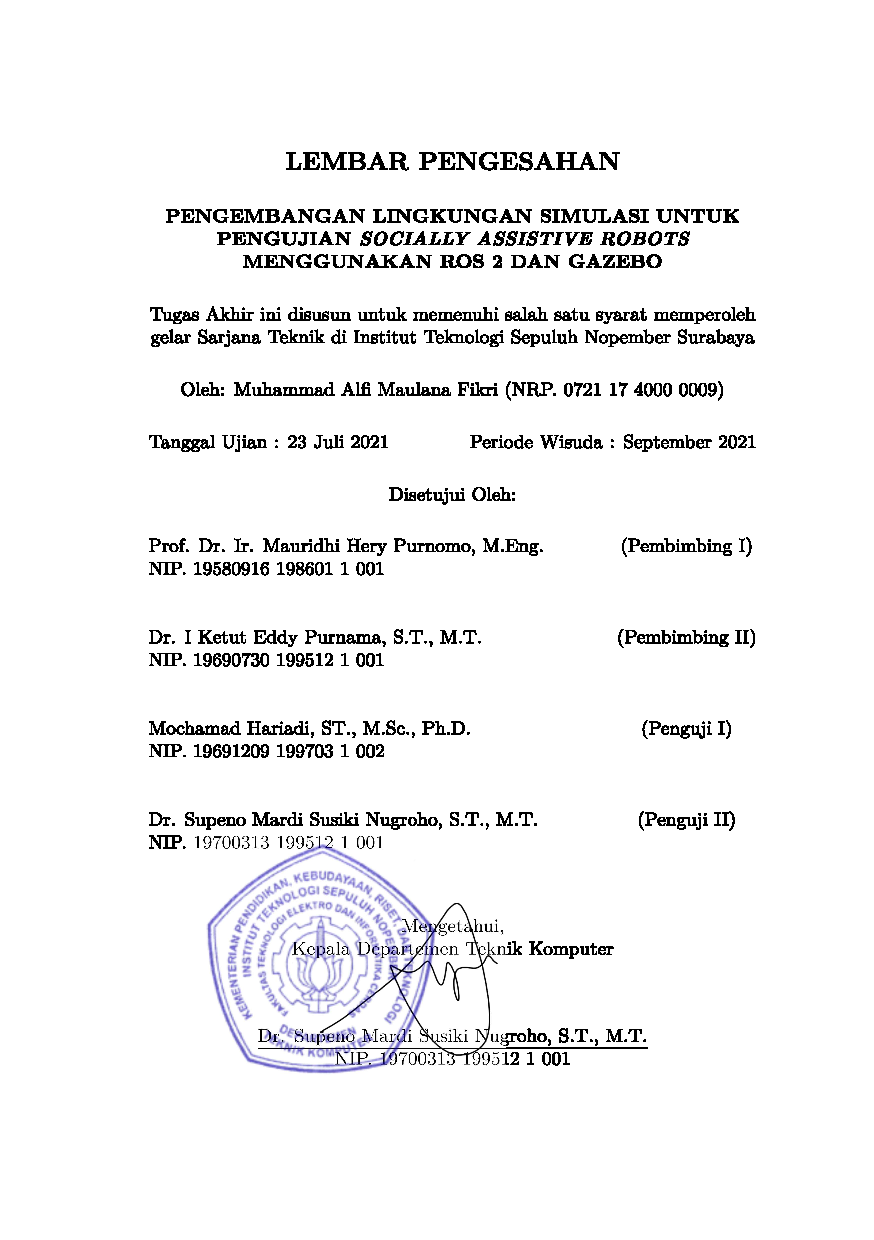
\includepdf{lainnya/lembar-pengesahan.pdf}
  % \newpage
  % \cleardoublepage

  \pagenumbering{roman}

  \phantomsection
  \addcontentsline{toc}{chapter}{ABSTRAK}
  \subimport{abstrak}{abstrak-id.tex}
  \cleardoublepage

  \phantomsection
  \addcontentsline{toc}{chapter}{ABSTRACT}
  \subimport{abstrak}{abstrak-en.tex}
  \cleardoublepage

  \phantomsection
  \addcontentsline{toc}{chapter}{KATA PENGANTAR}
  \subimport{lainnya}{kata-pengantar.tex}
  \cleardoublepage

  \renewcommand*\contentsname{DAFTAR ISI}
  \begin{spacing}{1} % Kurangi spasi di daftar isi
  \tableofcontents
  \addcontentsline{toc}{chapter}{\contentsname}
  \cleardoublepage

  \renewcommand{\listfigurename}{DAFTAR GAMBAR}
  \renewcommand{\cftloftitlefont}{\hfil\bfseries}
  % \renewcommand{\cftafterloftitle}{\hfil}
  \listoffigures
  \addcontentsline{toc}{chapter}{\listfigurename}
  \cleardoublepage
  % \renewcommand*\listfigurename{\hfill DAFTAR GAMBAR}
  % \renewcommand{\cftafterlottitle}{\hfill}
  % \listoffigures
  % \addcontentsline{toc}{chapter}{\listfigurename}
  % \cleardoublepage

  % \renewcommand*\lstlistlistingname{DAFTAR KODE}
  % \lstlistoflistings
  % \addcontentsline{toc}{chapter}{\lstlistlistingname}
  % \cleardoublepage

  % \renewcommand*\listtablename{\hfill DAFTAR TABEL}
  % \renewcommand{\cftafterlottitle}{\hfill}

  \renewcommand*\listtablename{\hfill \normalsize DAFTAR TABEL}
  \renewcommand{\cftafterlottitle}{\hfill}
  

  \listoftables
  \end{spacing}
  \addcontentsline{toc}{chapter}{\listtablename}
  \cleardoublepage

  \mainmatter
  % \pagenumbering{arabic}
  \setcounter{page}{1}
  
  \subimport{bab}{1-pendahuluan.tex}
  \cleardoublepage

  \subimport{bab}{2-tinjauan-pustaka.tex}
  \cleardoublepage

 \subimport{bab}{3-metodologi.tex}
 \cleardoublepage

 \subimport{bab}{4-analisis-pembahasan.tex}
 \cleardoublepage

  \subimport{bab}{5-penutup.tex}
  \cleardoublepage

  \renewcommand\bibname{DAFTAR PUSTAKA}
%  \setcitestyle{authoryear, open={(},close={)}}
  \bibliographystyle{apalike}
  \bibliography{pustaka/bibliografi.bib}
  \addcontentsline{toc}{chapter}{\bibname}
  \cleardoublepage

  \backmatter

  \appendix
  \renewcommand\thesection{Lampiran \arabic{section}}
  \subimport{lampiran}{lampiran-a.tex}

  \cleardoublepage
  \subimport{lainnya/}{biodata-penulis.tex}
\end{document}
